\documentclass[a4paper,11pt]{article}

\usepackage[german]{babel}
\usepackage[utf8]{inputenc}
\usepackage[T1]{fontenc}
\usepackage{listings}
\usepackage{booktabs}
\usepackage{hyperref}
\usepackage{enumitem}
\usepackage{graphicx}

\title{Technical Documentation: Vereinskassen-System}
\author{7157747, Gellien, 8425470, Heidusch}
\date{\today}

\begin{document}
\maketitle

\section{Analysis}

\subsection{Project Requirements}
Development of a virtual club treasury system with the following key features:
\begin{itemize}
\item User authentication system with different roles
\item Department account managemen
\item Transaction handling and history tracking
\item Balance monitoring and prevention of negative balances
\item Data persistence using CSV files
\end{itemize}

\subsection{System Architecture}
\subsubsection{Model-View-Controller (MVC) Pattern}
The system implements the MVC pattern:
\begin{itemize}
\item Models: User, Account, Transaction, UserRole
\item Views: MainView, LoginView, AdminView, TreasurerView, FinanceView
\item Controllers: AuthController, TransactionController
\end{itemize}

\subsection{Data Structure}
\subsubsection{CSV File Structure}
\begin{itemize}
\item users.csv: username, password, role, department
\item accounts.csv: accountid, department, balance, treasurer
\item transactions.csv: transactionid, timestamp, amount, type, source, target, description
\end{itemize}

\begin{figure}[h]
    \centering
    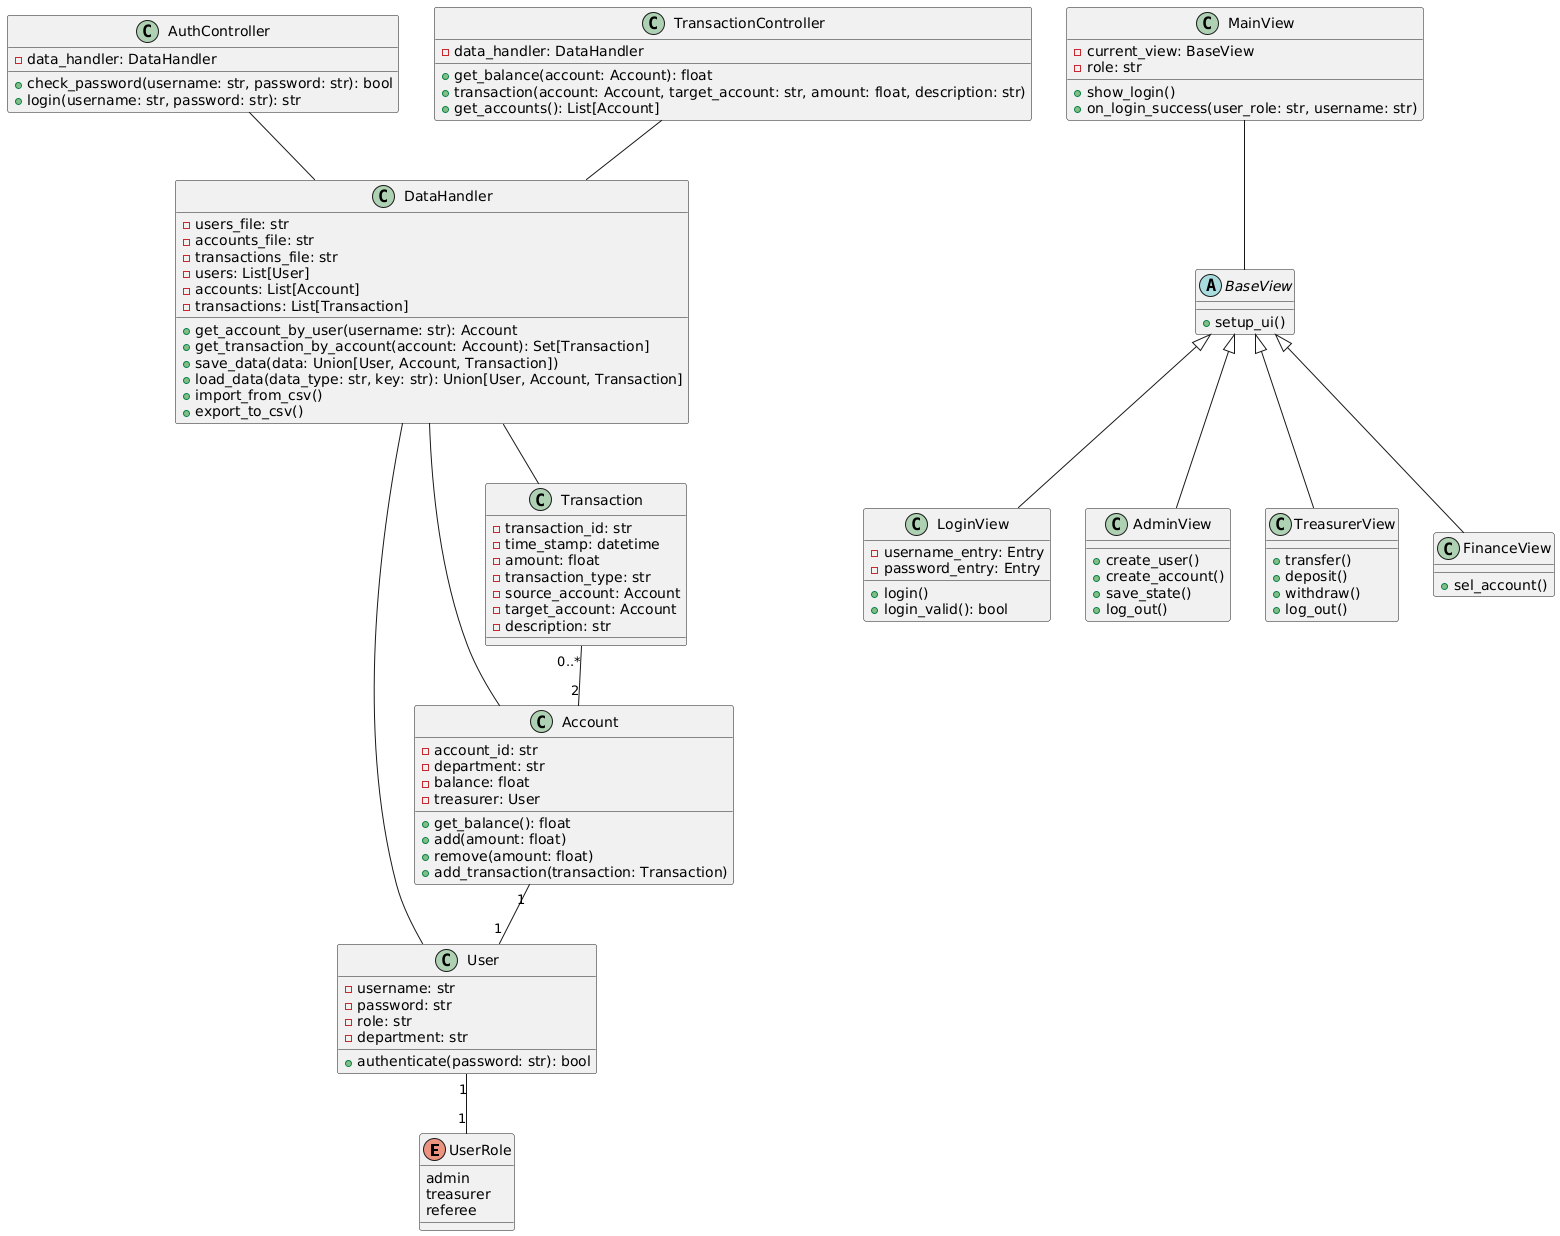
\includegraphics[width=\textwidth]{uml.png}
    \caption{Class Diagram of the Vereinskassen-System}
    \label{fig:uml}
\end{figure}

The UML class diagram (Figure \ref{fig:uml}) illustrates the system's architecture following the Model-View-Controller pattern:

\section{Implementation}

\subsection{Key Classes}
\begin{itemize}
\item \textbf{DataHandler}: Manages data persistence and retrieval
\item \textbf{User}: Handles user authentication and permissions
\item \textbf{Account}: Manages account balances and transactions
\item \textbf{Transaction}: Records financial transactions
\end{itemize}

\subsection{Controllers}
\begin{itemize}
\item \textbf{AuthController}: Manages user authentication and authorization
\item \textbf{TransactionController}: Handles financial transactions and balance updates
\end{itemize}

\subsection{Views}
\begin{itemize}
\item \textbf{MainView}: Primary application window
\item \textbf{LoginView}: User authentication interface
\item \textbf{AdminView}: Administrator management interface
\item \textbf{TreasurerView}: Department account management interface
\item \textbf{FinanceView}: Financial overview interface
\end{itemize}

\section{Testing}

\subsection{Test Cases}

\subsubsection{Authentication Tests (TestAuthController)}
\begin{itemize}
\item \textbf{test\_check\_password}
  \begin{itemize}
  \item Purpose: Verify password verification functionality
  \item Test Data: User "hanz" with password "1234"
  \item Expected Result: Password check returns True
  \item Status: Passed
  \end{itemize}

\item \textbf{test\_login}
  \begin{itemize}
  \item Purpose: Verify login process and role assignment
  \item Test Data: User "hanz" with admin role
  \item Expected Result: Login returns correct user role
  \item Status: Passed
  \end{itemize}
\end{itemize}

\subsubsection{Data Handling Tests (TestDataHandler)}
\begin{itemize}
\item \textbf{Data Creation Tests}
  \begin{itemize}
  \item \textbf{test\_add\_user}
    \begin{itemize}
    \item Purpose: Verify user creation and storage
    \item Test Data: Admin user "hanz"
    \item Expected Result: User correctly stored in users list
    \item Status: Passed
    \end{itemize}

  \item \textbf{test\_add\_account}
    \begin{itemize}
    \item Purpose: Verify account creation and storage
    \item Test Data: Account "abc" with balance 0.4
    \item Expected Result: Account correctly stored in accounts list
    \item Status: Passed
    \end{itemize}

  \item \textbf{test\_add\_transaction}
    \begin{itemize}
    \item Purpose: Verify transaction creation and storage
    \item Test Data: Transaction between two accounts
    \item Expected Result: Transaction correctly stored in transactions list
    \item Status: Passed
    \end{itemize}
  \end{itemize}

\item \textbf{Data Retrieval Tests}
  \begin{itemize}
  \item \textbf{test\_load\_user}
    \begin{itemize}
    \item Purpose: Verify user retrieval functionality
    \item Test Data: User "franz"
    \item Expected Result: Correct user object returned
    \item Status: Passed
    \end{itemize}

  \item \textbf{test\_load\_account}
    \begin{itemize}
    \item Purpose: Verify account retrieval functionality
    \item Test Data: Account "abc"
    \item Expected Result: Correct account object returned
    \item Status: Passed
    \end{itemize}

  \item \textbf{test\_load\_transaction}
    \begin{itemize}
    \item Purpose: Verify transaction retrieval functionality
    \item Test Data: Transaction "ab"
    \item Expected Result: Correct transaction object returned
    \item Status: Passed
    \end{itemize}
  \end{itemize}

\item \textbf{Data Persistence Test}
  \begin{itemize}
  \item \textbf{test\_export\_import}
    \begin{itemize}
    \item Purpose: Verify CSV export and import functionality
    \item Process: Export data, clear memory, import data
    \item Expected Result: All data correctly persisted and retrieved
    \item Status: Passed
    \end{itemize}
  \end{itemize}
\end{itemize}

\subsection{Test Environment}
\begin{itemize}
\item Test files located in tests/files/
\item Separate CSV files for test data
\item Clean file state maintained between tests
\end{itemize}



\subsection{Test Data}
Test files located in tests/files/:
\begin{itemize}
\item usersfile.csv
\item accountsfile.csv
\item transactionsfile.csv
\end{itemize}

\section{Setup and Dependencies}
\begin{itemize}
\item Python 3.12
\item Tkinter for GUI
\item Setup via setup.py
\item Project structure follows standard Python package layout
\end{itemize}

\end{document}
